\subsection{Example: Four-bar linkage Mechanism}

\begin{frame}
	\begin{block}{Example 2: Four-bar linkage Mechanism}
		\begin{table}
			\begin{minipage}{0.5\linewidth}
				\begin{tabular}{l|l}
					& $l_{AB}=l_1=0.15m$\\
					& $l_{BC}=l_2=0.35m$\\
					& $l_{CD}=l_3=0.3m$\\
					Given & $l_{CE}=l_4=0.15m$\\
					& $x_D=0.3m$\\
					& $y_D=0.3m$\\
					& $\theta_1=45^ {\circ}$\\ \hline
					Find & $\vb{r}{B}$, $\vb{r}{C}$, $\vb{r}{E}$\\
				\end{tabular}	
			\end{minipage}\hfill
			\begin{minipage}{0.5\linewidth}
				\begin{figure}
					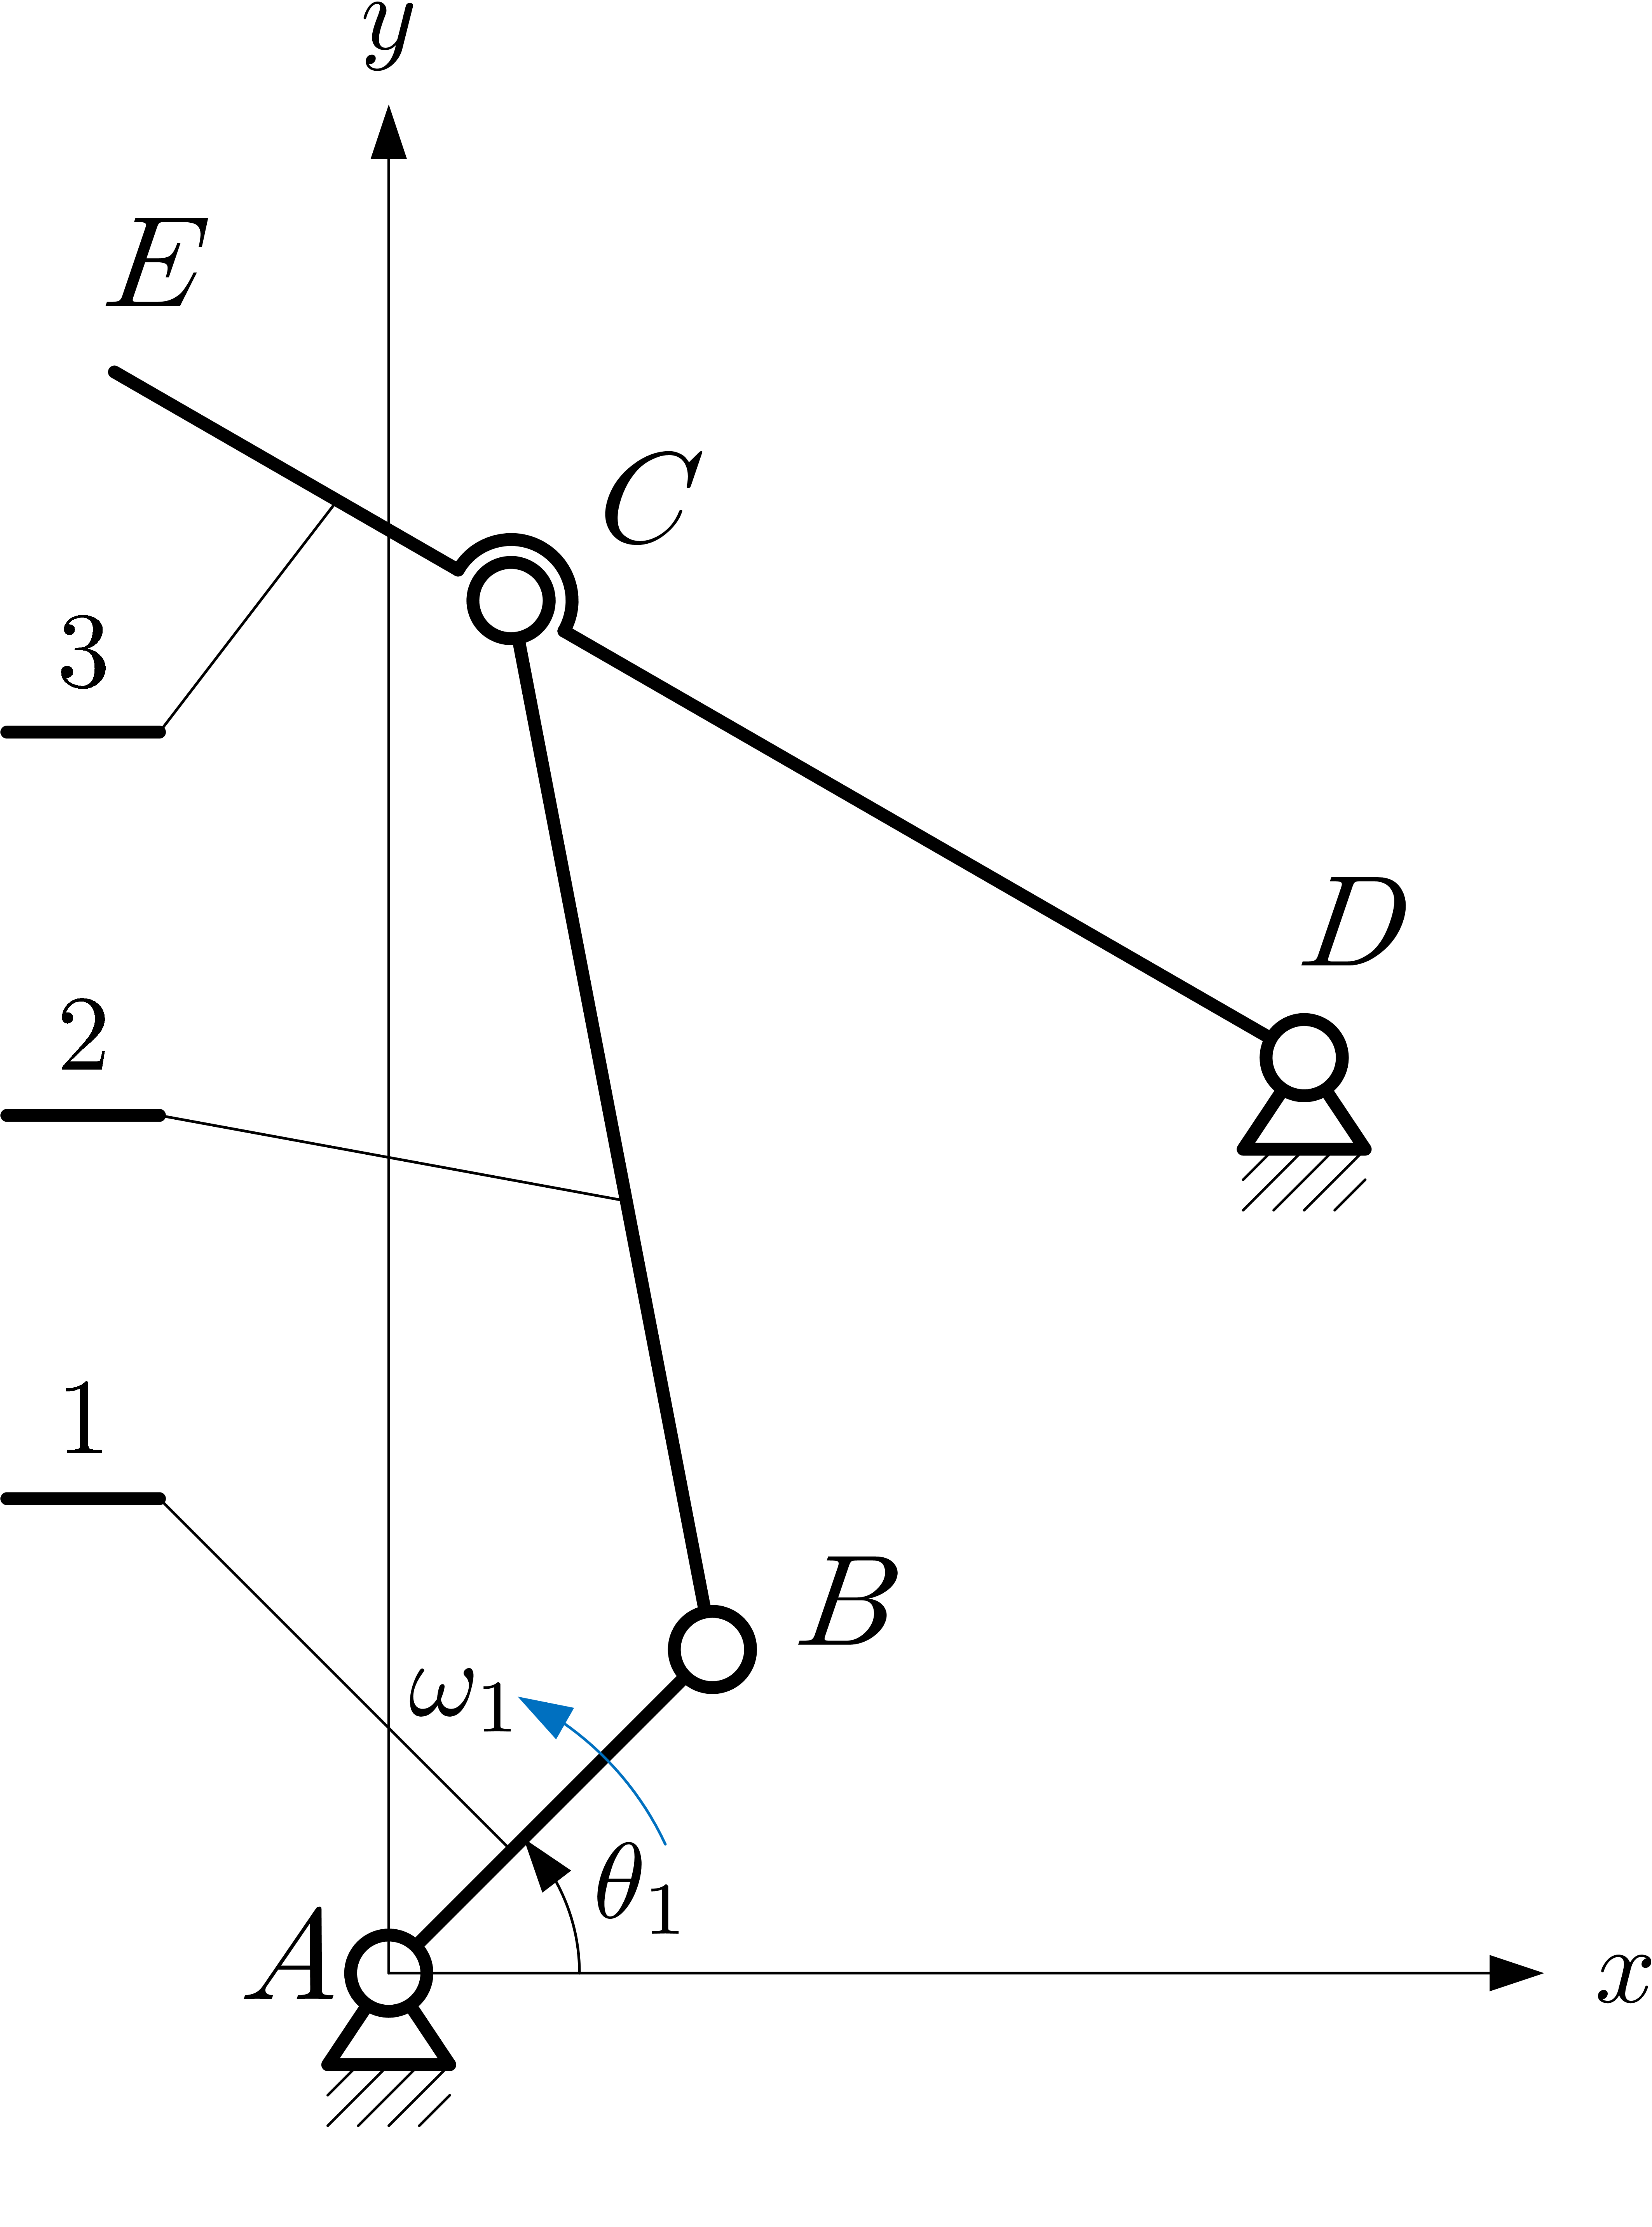
\includegraphics[width=50mm]{images/R-RRR.png}
				\end{figure}
			\end{minipage}
		\end{table}
	\end{block}
\end{frame}

\begin{frame}
\emph{Solution}\vskip .25cm
Position of joint $B$:  $\displaystyle \vb{r}{B} = x_B\ih + y_B\jh = l_1\cos{\theta_1}\ih + l_1\sin{\theta_1}\jh$\\
Position of joint $C$:  $\displaystyle \vb{r}{C} = x_C\ih + y_C\jh = 0.1\jh$\\
Position of joint $D$: $\displaystyle \vb{r}{D} = x_D\ih + y_D\jh$\\
Position of joint $E$: $\displaystyle \vb{r}{E} = x_E\ih + y_E\jh$\\
\[
\Rightarrow\begin{cases}
(x_B-x_C)^2+(y_B-y_C)^2=l_1^2\\
(x_D-x_C)^2+(y_D-y_C)^2=l_3^ 2
\end{cases}
\]
Solving the system of equations yields $x_{C_1}$ and $x_{C_2}$. Notice that in the mechanism, $0>x_C$ is the condition to obtain correct solution.
\[
\Rightarrow \begin{cases}
(x_C-x_E)^2 + (y_C-y_E)^2 = l_4^2\\
\displaystyle \frac{y_C-y_E}{x_C-x_E}=\frac{y_D-y_E}{x_D-x_E}
\end{cases}
\]
Solving the system of equations yields $x_{E_1}$ and $x_{E_2}$. Notice that in the mechanism, $x_C>x_E$ is the condition to obtain correct solution.
\end{frame}


\begin{frame}{MATLAB R2019a code}
\lstinputlisting[style=Matlab-editor, basicstyle=\mlttfamily]{codes/RRRR-position1.m}
\end{frame}
\begin{frame}
\lstinputlisting[style=Matlab-editor, basicstyle=\mlttfamily]{codes/RRRR-position2.m}
\end{frame}
\begin{frame}{Plotting using MATLAB R2019a}
\lstinputlisting[style=Matlab-editor, basicstyle=\mlttfamily]{codes/RRRR-plot.m}
\end{frame}
\begin{frame}{Output figure}
\centering
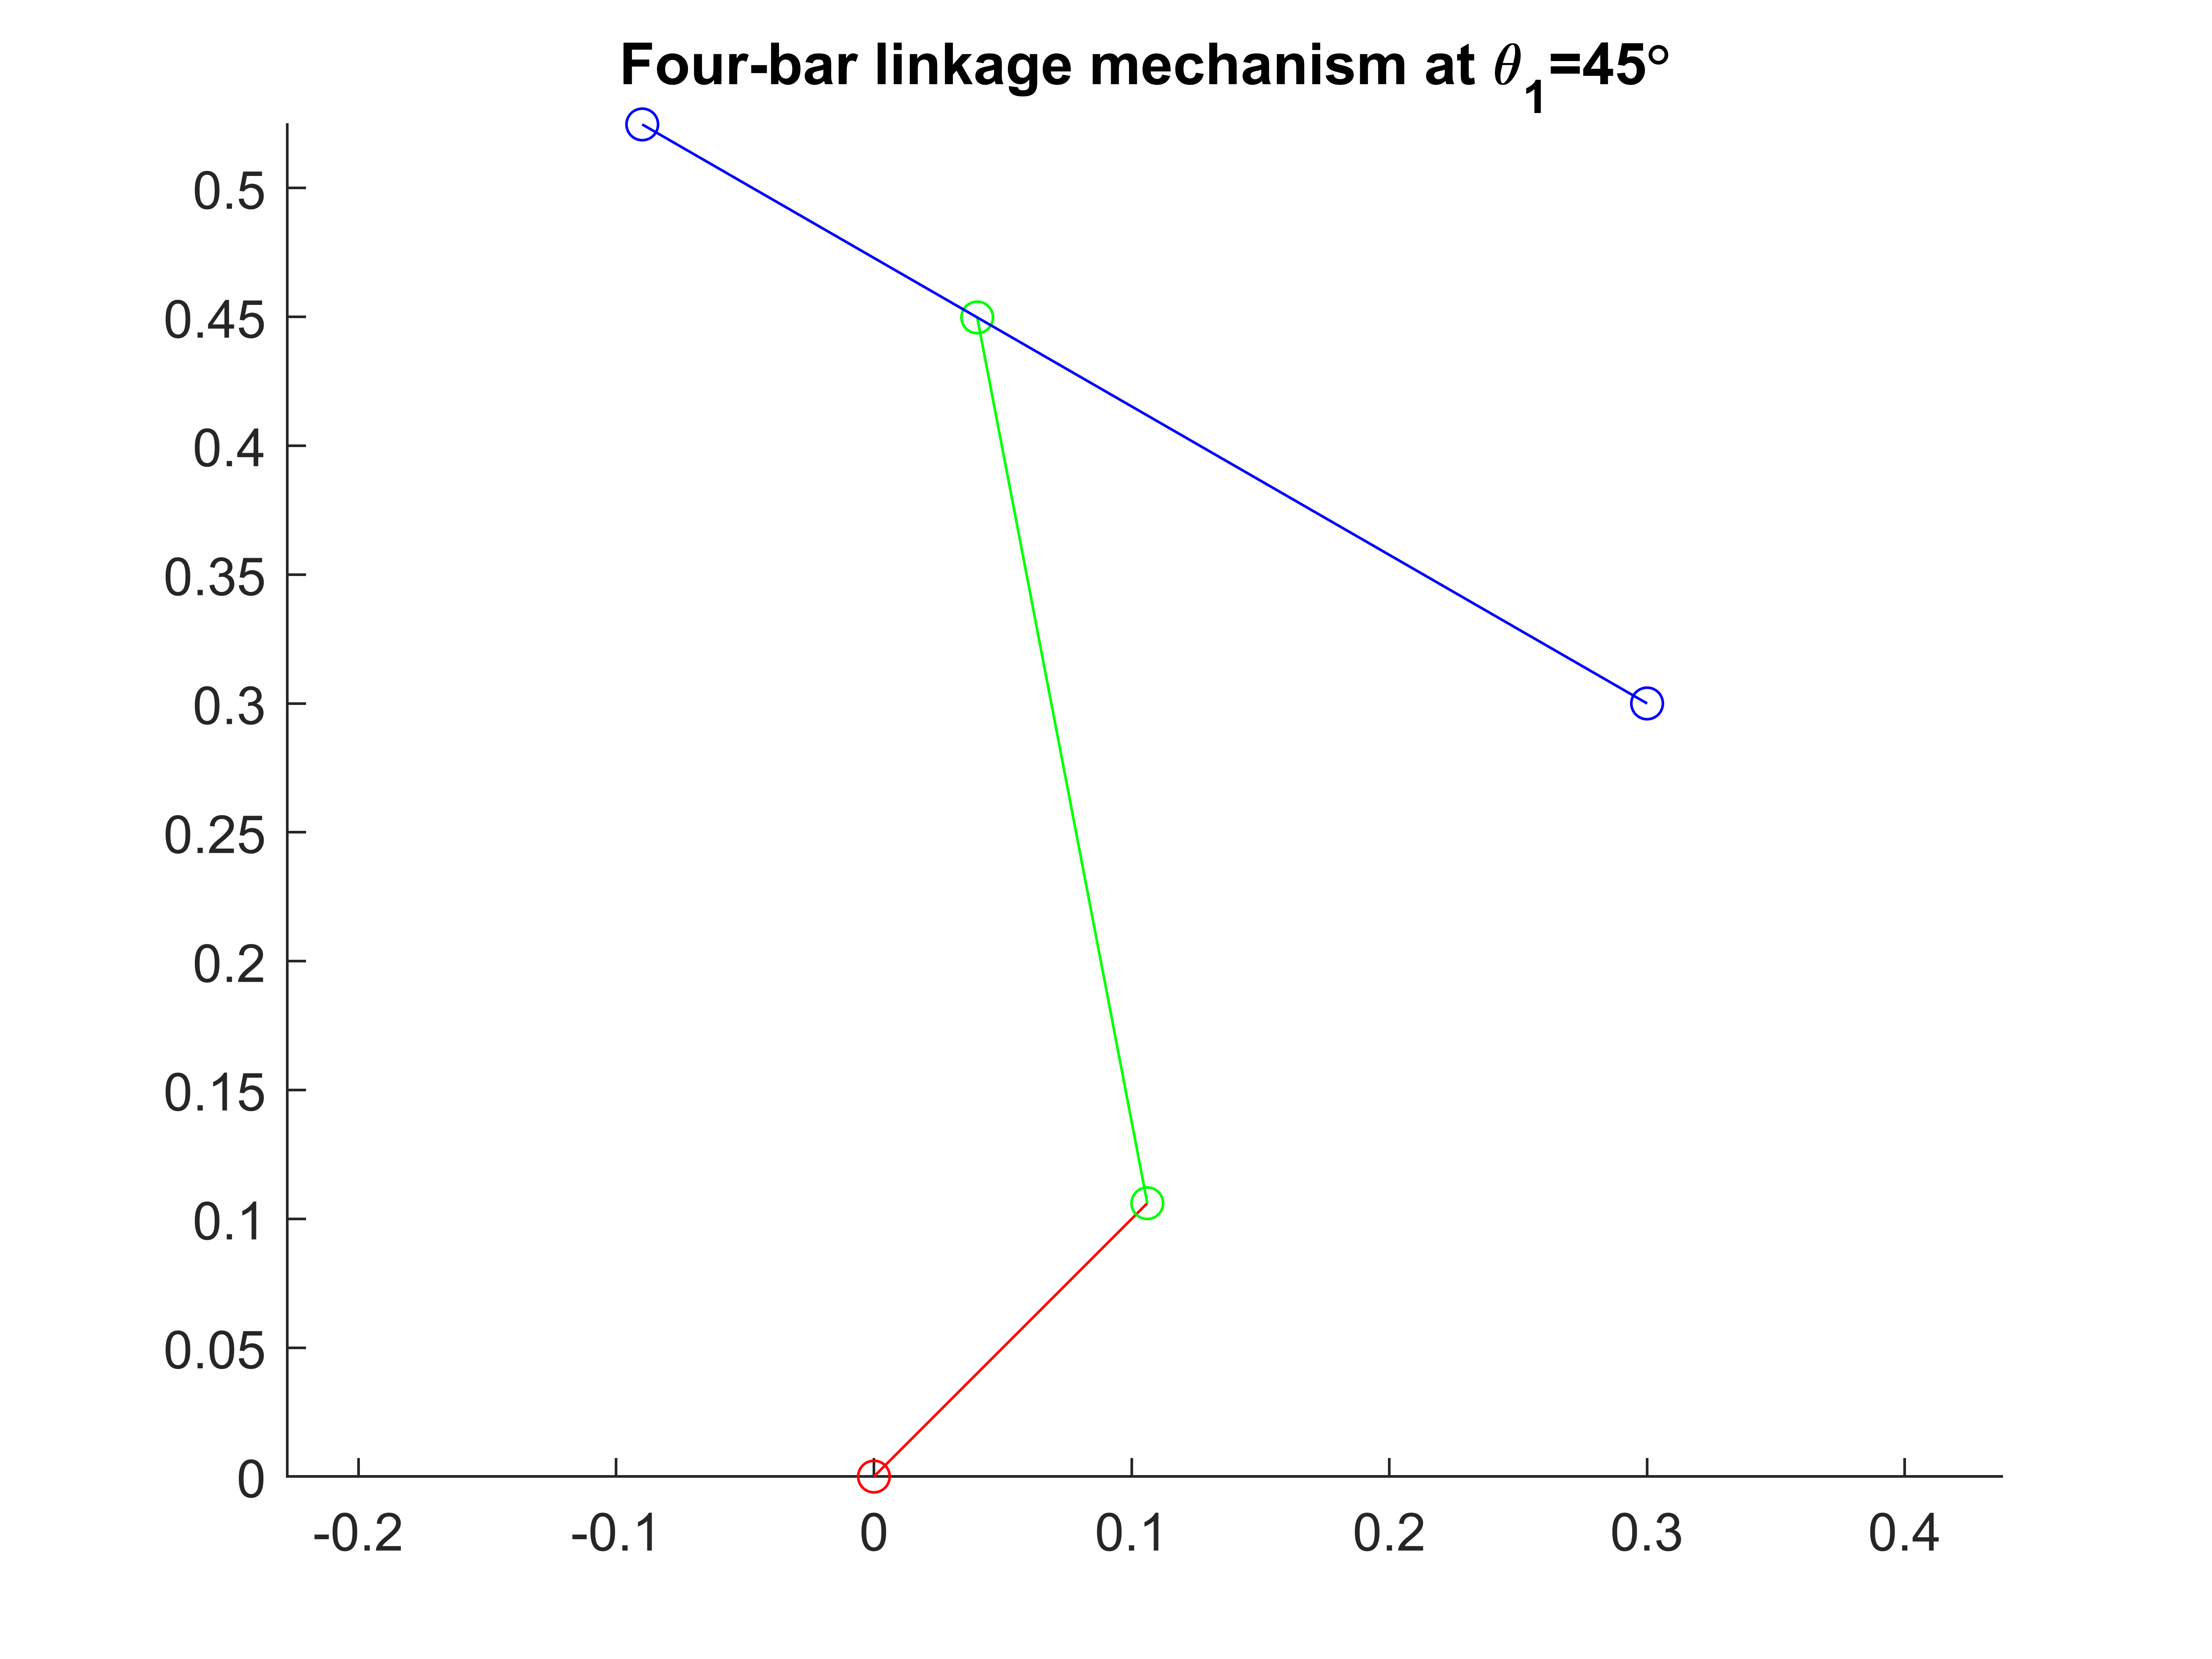
\includegraphics[width=100mm]{images/RRRR-plot.png}
\end{frame}
\begin{frame}{Trajectory plotting using MATLAB R2019a}
\lstinputlisting[style=Matlab-editor, basicstyle=\mlttfamily]{codes/RRRR-trajectory.m}
\end{frame}
\begin{frame}{Output figure}
\centering
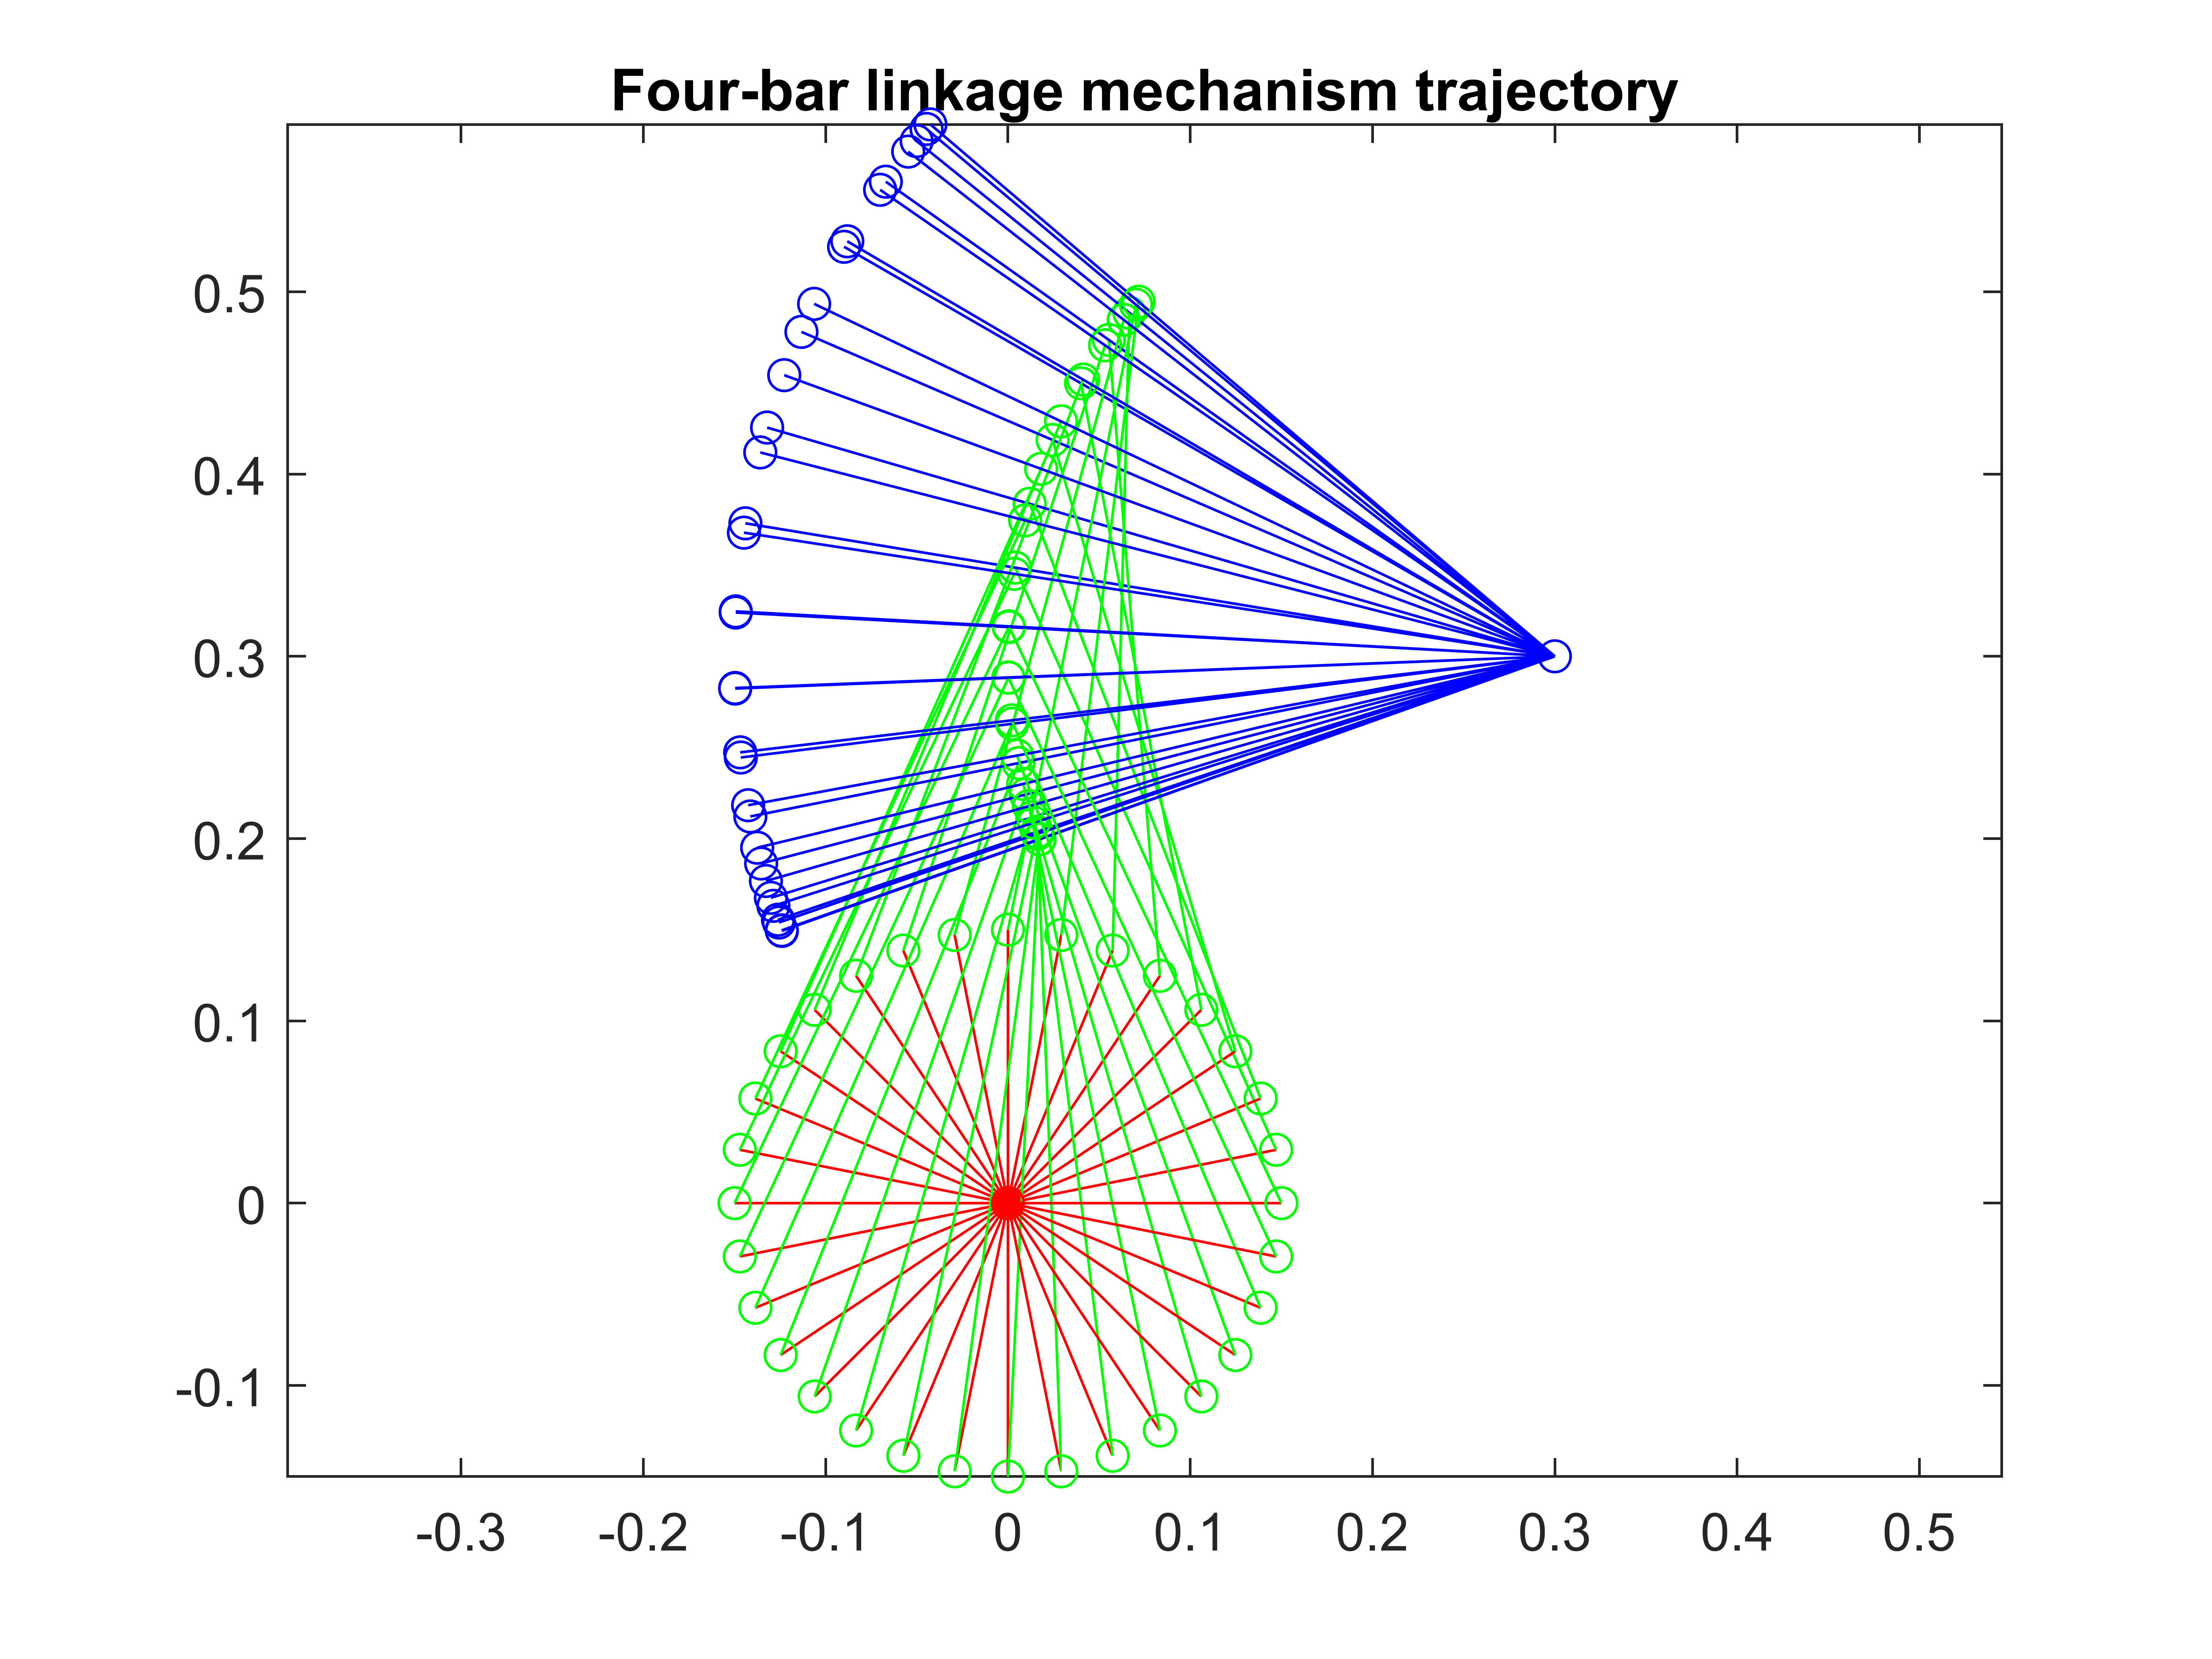
\includegraphics[width=100mm]{images/RRRR-trajectory.png}
\end{frame}